\begin{figure*}[ht]
\centering
\subfigure{
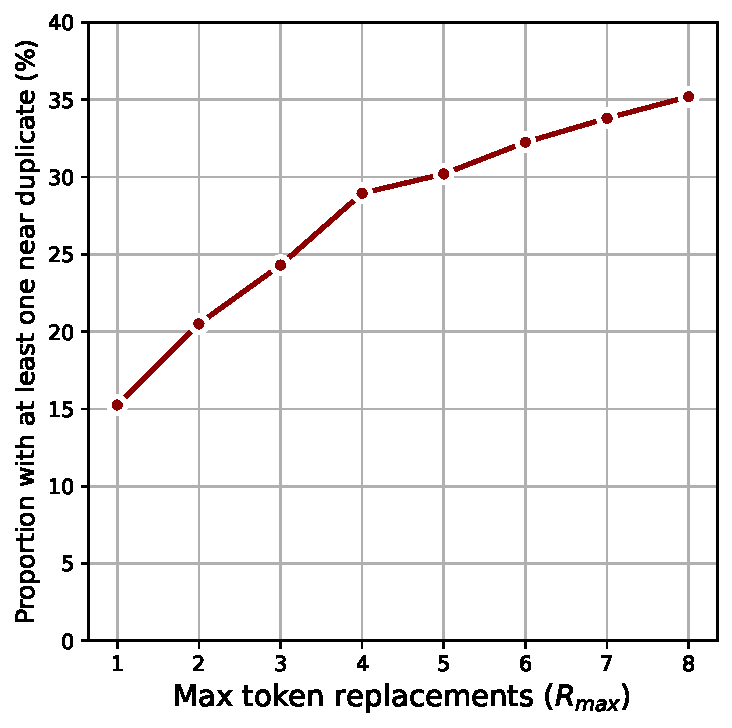
\includegraphics[width=0.4\linewidth]{figures/near_duplicates_proportion.pdf}
}
\subfigure{
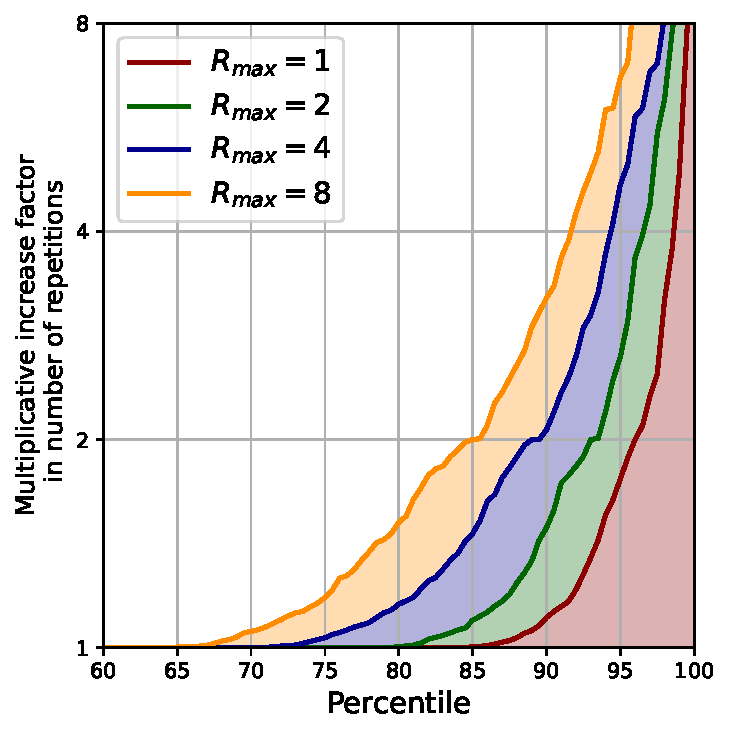
\includegraphics[width=0.4\linewidth]{figures/near_duplicates_percentiles.pdf}
}
\caption{\textbf{Fuzzy duplicate sequences in The Pile.} (a) Proportion of sequences with at least one fuzzy duplicate given the maximum threshold $R_\text{max}$ (b) An increase in total number of repetitions if accounting for fuzzy duplicates given the maximum threshold $R_\text{max}$.}
\label{fig:near_dups}
\end{figure*}


Prior work on memorization in LLMs often relies on the natural presence of the duplicated sequences in large text datasets~\cite{carlini2021extracting,carlini2022quantifying,kandpal2022deduplicating, ippolito2022preventing}. For instance, seminal work by Carlini et al.~\cite{carlini2022quantifying} identifies sequences repeated multiple times in The Pile~\cite{pile}, and uses this to study the relationship between the number of repetitions and memorization. Kandpal et al.~\cite{kandpal2022deduplicating} adopts a similar approach with C4~\cite{2019t5} and OpenWebText~\cite{Gokaslan2019OpenWeb}.

We argue that relying on naturally occurring duplicates might overestimate the impact of exact duplication on memorization. Instead, some memorization could be attributed to fuzzy duplicates. Any memorization study using the set of exact duplicates found in a large text dataset is susceptible to the confounding factor from the presence of fuzzy duplicates. As we show below, the number of fuzzy duplicates tend to be distributed in a highly non-uniform fashion, likely introducing bias when studying memorization.

To verify this, we here re-create the set of sequences duplicated in The Pile considered by prior work. We use the code provided by Lee et al.~\cite{lee2022deduplicating}\footnote{Distributed under Apache License 2.0.} to build a suffix array and identify sequences occurring at least twice in the dataset. We consider sequences of 100 BPE (GPT-2) tokens~\cite{radford2019language}. As the original The Pile has been taken down due to copyright violations in some of its subsets, we study the non-copyrighted version of The Pile~\cite{pile_uncopyrighted}, which covers roughly 80\% of the original data\footnote{The rest of The Pile is distributed under a range of permissive licences.}. While this affects the absolute counts of exact and fuzzy duplicates, we effectively report the lower bound on both counts, which allows us to study their relative prevalence in large datasets. Data processing took us $\sim96$ hours on a machine with 96 CPUs, 500GB of RAM and 5TB of available disk space.

Following the approach proposed by Carlini et al.~\cite{carlini2022quantifying}, we group duplicate sequences into buckets by the number of exact repetitions, where the $n$-th bucket contains sequences repeated between $2^{n/4} \leq n_{dup} < 2^{(n+1)/4}$ times in the dataset. We consider $n \in [20, 40)$, thus covering sequences repeated between $32$ and $1024$ times. We then sample $100$ random sequences from each bucket (2000 sequences overall) and search for their fuzzy duplicates. As in the experiments above, we define a fuzzy duplicate as a sequence of the same length with up to a certain number of tokens ($R_\text{max}$) replaced between the two sequences (we consider $R_\text{max} \leq 8$). Note that the notion of the number of tokens replaced between two sequences of the same length is equivalent to the Hamming distance - we here adopt the former for consistency.  
For computational reasons, we only look for fuzzy duplicates among sequences identified as duplicates themselves, i.e. repeated in the original dataset at least twice. Our fuzzy duplicate counts, therefore, only provide a lower bound estimation of the total number of fuzzy duplicates for a given sequence.

Our results show that a significant proportion of sequences duplicated in The Pile have additional fuzzy duplicates in the dataset. Fig.~\ref{fig:near_dups}(a) shows that almost 15\% and 30\% of sequences have at least one fuzzy duplicate with only a $R_\text{max}=1$ and $R_\text{max}=4$ token replacements respectively (out of a 100 tokens in the sequence). Strikingly, Fig.~\ref{fig:near_dups}(b) shows that for 10\% of all duplicate sequences, the number of fuzzy duplicates ($R_\text{max}=4$) is larger than the number of exact repetitions. For instance, 10\% of all sequences repeated $32$ times in The Pile have more than $32$ additional fuzzy duplicates. This data suggests that using naturally occurring duplicates to study memorization is prone to unforeseen confounding factors, such as the presence of fuzzy duplicates illustrated above.